\chapter{Experiments}
The main purpose of this chapter of this paper is to compare animations
generated procedurally with the use of Ik with baked animations. The comparison
is broken up into two categories - visual and performance. 

\section{Baked animations}
 In order to conduct the experiments comprised of visual and performance
 comparisons, a second set of animations were created each of the examples which
 are shown in the demo application. Below is an explanation of the process of
 creating this second set of animations.

\subsubsection{Spider}
The baked animation version of the spider was animated in Blender. The set
consists of idle and walking animations which, in Blender, are placed on
a single timeline, one after the other (Figure \ref{fig:timeline}). Once the model is imported
into Unity, the animations can be broken up into their separate cases, as shown
earlier in the "tools" chapter of this paper (Figure \ref{fig:anim_chunk}). 

\begin{figure}[h!]
    \centering
    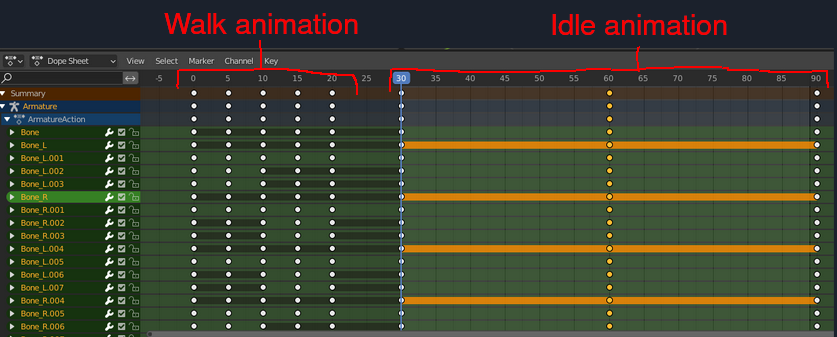
\includegraphics[width=0.7\textwidth]{grafika/blender_timeline.png}
    \caption{Two animations on a single timeline}
    \label{fig:timeline}
\end{figure}

Once the animations have been imported, a new animation controller was created
for the new spider. The animations are added, this time with the use of a blend
tree (Figure \ref{fig:s_blendtree}) to, as the name suggests, blend between the
animation smoothly CITE. A third animation state is added to the blend tree
which is the equivalent of the walking animation, but the animation speed is set
to a negative value. This plays the animation in reverse and is used when the
spider is walking backwards. 

\begin{figure}[h!]
    \centering
    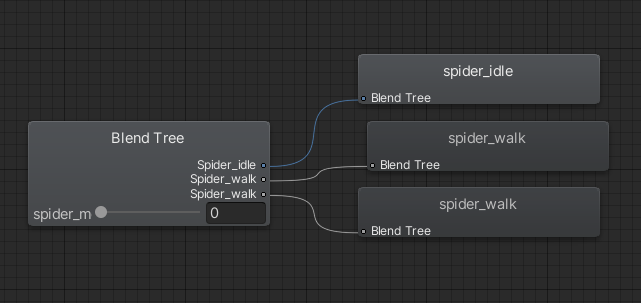
\includegraphics[width=0.7\textwidth]{grafika/spider_blend.png}
    \caption{Blend tree containing animations for the spider}
    \label{fig:s_blendtree}
\end{figure}

A variable named \textit{spider\_movement} is created in order to control the
animations that are to be played in a given situation, and the manner in which
the transitions should be blended. The thresholds for each animation can be
defined in the blend tree's configuration in the animator (Figure ref).

\begin{figure}[h!]
    \centering
    \captionsetup{justification=centering}
    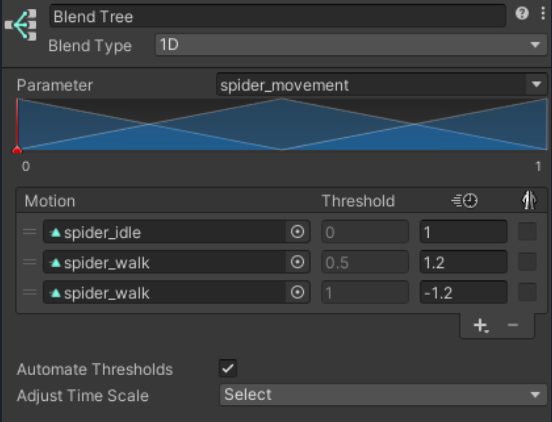
\includegraphics[width=0.7\textwidth]{grafika/spider_blendconf.png}
    \caption{Configuration of the spider's blend tree which is dependent on
    the \textit{spider\_movement} variable}
    \label{fig:s_blendconf}
\end{figure}

In the spiders movement script, this variable can then be set in reaction to
certain inputs so that the proper animation is activated each given situation.
To achieve the transition blending, the \textit{spider\_movement} variable
should not be set outright to the value which corresponds to the next animation
state. Instead, the \textit{\_animator.SetFloat} method is used, where the
\textit{\_animator} is a reference to the spider's Animator component. This
method allows the value of spider\_movement to be interpolated from the value of
the current animation state to another desired value.
\newline
\begin{lstlisting}[basicstyle=\footnotesize, numbers=none,frame=single,
caption={Transitioning to the spider's idle animation using the
\textit{SetFloat} method},captionpos=b, label=stretch, language={[Sharp]c}]
    if (verticalAxis == 0f && horizontalAxis == 0f)
        _animator.SetFloat("spider_movement", 0f, 0.05f, Time.deltaTime);
\end{lstlisting}

This version of the spider has its movement based on the spider from the game
Minecraft, which means that its rotation on the x and z axes is locked. The
spider can rotate about the y-axis when turning to face a different direction,
but it will not adjust to variations in the surface which it walks upon.
Additionally, when the spider encounters a vertical wall, it begins moving
vertically instead of horizontally until it scales the entire obstacle.

\subsubsection{Human}
The baked version of the human character which performs an animation sequence
consisting of pressing buttons is also animated in Blender. The animation plays
one full sequence of pressing a single button. Chunks of the same animation are
used in the IK version of this animation sequence which is described in the
previous chapter, however the baked animation utilizes the full animation while
the IK version uses only the beginning and the end. Nevertheless, the animation
is still broken up into three parts when imported into Unity: the raising of the
hand, the button pressing motion, and the lowering of the hand.


